\chapter*{Foreword on Methodology}
\thispagestyle{empty}
\addcontentsline{toc}{chapter}{Foreword on Methodology}

As we explained in Section~\ref{sec:webrtc}, WebRTC is a set of standard specifications aiming to provide to webpages the capability to setup \gls{voip} communications.
These specifications also rely on other standards and techniques: authentication delegation protocols, \gls{voip} protocols and archirectures, JavaScript \gls{api}, cryptography, ...
At the heart of the WebRTC identity architecture is the proposal of an abstract authentication interface for peer-to-peer authentication and the claim that trust in an \gls{idp} can replace trust in the signalling path. 
We aim to study these propositions and at the same time answer our research questions.
However, we believe that formal paper-based study of standards must be conducted in conjunction with study of running implementations, in a complementary approach.
Indeed, standards are ultimately implemented in actual running code.
During this continuous process, implementors may take liberties with the specification, add non-standard functionalities, or decide to not implement some of them.
Furthermore, cross-implementation issues may arise, in particular when the integration of two specifications has not been thoroughly considered.
This is precisely the case of the WebRTC identity architecture which only sketches the OAuth~2 protocol integration.
It appears that, from our state of the art survey in Chapter~\ref{sota}, most of the researches on WebRTC security have been conducted without considering actual implementations.

\begin{figure}[H]
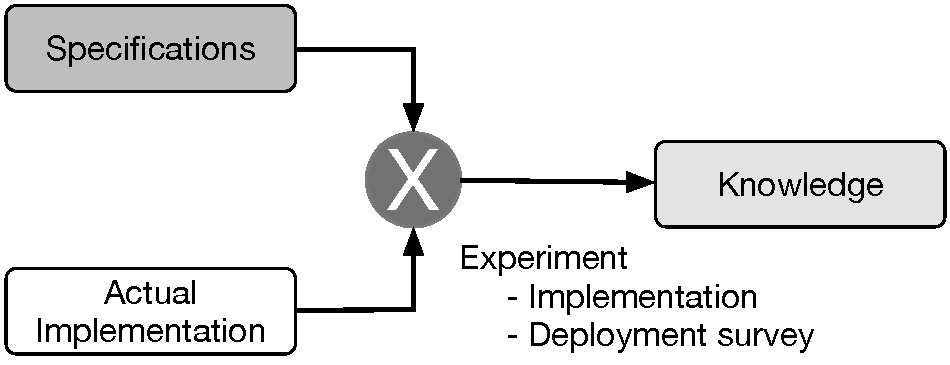
\includegraphics[scale=.5]{images/science}
\caption{Overview of our Scientific Methodology}
\label{science}
\end{figure}

Our approach, which we schematise in Figure~\ref{science}, differs.
The first step of our work is to conduct a study of these standards and techniques.
We presented the results of this step in Chapter~\ref{security}~and~\ref{sota}.
However, we then use actual implementations to answer our research questions. 
To do so, we conduct two types of experiments:
\begin{itemize}
\item In implementation experiments we develop software to put an already specified or a new functionality into action.
This allows us to discover actual issues encountered during the implementation and integration processes.
We describe our implementations so that our experiments can be reproduced~\footnote{The description of our implementations may also be helpful for developers facing similar needs.}.
\item In deployment survey experiments, we observe whether a functionality is implemented or used in existing and deployed softwares.
Observing an exposed functionality demonstrates if and how it can be used, while observing its actual usage reveals its importance for other services.
\end{itemize}

These experiments form the basis of our scientific methodology which we apply in the following contribution chapters.



\chapter{Privacy Implications of the WebRTC Identity Architecture}
\label{webrtcprivacy}
\begin{quote}
\textit{
A claim of the WebRTC security architecture specification~\cite{I-D.ietf-rtcweb-security-arch} is that trust in the signalling layer can be replaced by trust in the \gls{idp}.
This has implications regarding potential privacy issues.
As signalling and identity functions are decoupled, a new actor (the \gls{idp}) is introduced in the communication setup.
Even-though \gls{idp} already occupy a central role on the Web, their role in WebRTC has the potential to reinforce their position.
In this chapter, we study the privacy implications of the WebRTC Identity Architecture.
This part of the WebRTC specification lacks support on web browsers.
To the best of our knowledge, there is no publicly implementation or deployment of a WebRTC identity enabled WebRTC service or of an \gls{idp} supporting the WebRTC identity architecture.
To better understand the WebRTC Identity Architecture, it is thus necessary to first implement it.
We describe our implementations in Section~\ref{idpproxyimplem}.
We then detail additional privacy considerations in Section~\ref{sec:privacyissue}.
One issue we observe is that the \gls{idp} choice is limited by the \gls{cs} which may appear contradictory with the initial objective of the specification.
In Section~\ref{userschooseidp} we study why users cannot choose their \gls{idp} on the Web. 
}
\end{quote}

\begin{figure}[H]
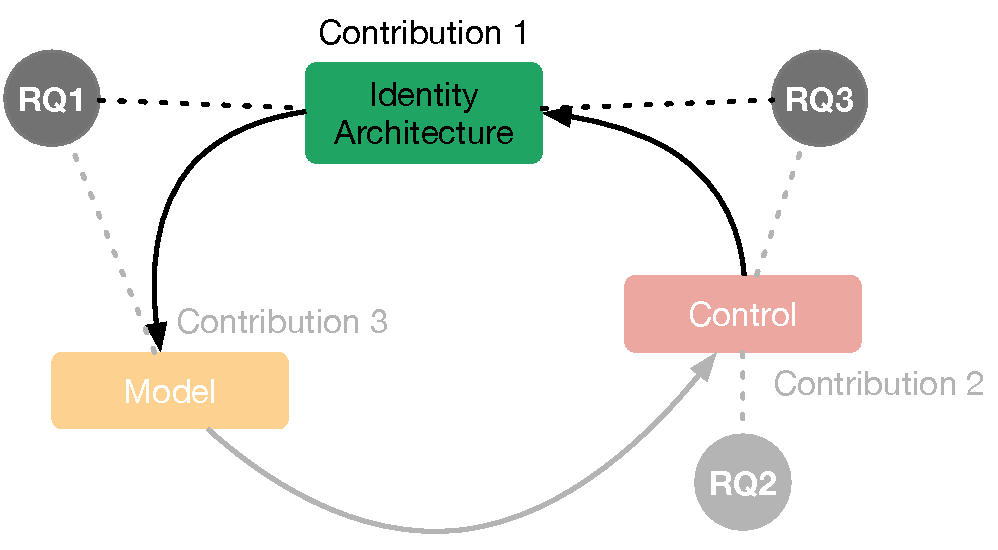
\includegraphics[scale=.5]{images/contrib1}
\caption{Overview of our Contributions: Study of the WebRTC Identity Architecture.}
\label{contrib1}
\end{figure}


\glsresetall
\section{WebRTC Identity Architecture Implementation}
\label{idpproxyimplem}
The explicit peer authentication proposed by the WebRTC specification plays a central part of the WebRTC identity architecture.
But it is also, for the moment, a feature whose implementation in browser lags behind others WebRTC features.
The \texttt{RTCPeerConnection} identity interface is only implemented in Firefox.
As a result and to the best of our knowledge, no \gls{idp} or WebRTC service are supporting it\footnote{\url{https://bugs.chromium.org/p/chromium/issues/detail?id=493640}}.
Our first research question (RQ1) consists in understanding the risk for the user of a WebRTC session. 
More particularly, in this section we address the following question:
\begin{itemize}
\item \textbf{RQ1.1}: Are there any security vulnerabilities in the identity path of the WebRTC security architecture?
\end{itemize}
We want to validate our work on a running implementation of the WebRTC identity architecture.
To do so, we develop a simple WebRTC service\footnote{\url{https://github.com/Sparika/ACOR\_SDP}} offering communication for two users in a single room.
The communication server is built with the NodeJS framework.
Session signalling is done through the \gls{cs} server over web sockets and the JavaScripts client code manages the call session.
We conduct our tests on Firefox version 50.1.0. 

As the RTCPeerConnection identity interface is provided by Firefox, the missing part of the WebRTC identity architecture is an \gls{idp} exposing \gls{idp} Proxy.
In addition to a WebRTC service, we also implement \gls{idp} Proxies for three different \gls{idp}, following the WebRTC specification.
The first \gls{idp} is actually our WebRTC communication service itself in what we call a local authentication scenario.
We present this implementation in Section~\ref{sec:idpstd}.
Our two other \gls{idp} Proxies are developed for two OIDC servers.
The first server is one of the reference implementations by Nat Sakimura\footnote{\url{https://github.com/reTHINK-project/dev-IdPServer-phpOIDC}}, while the second one is an implementation in NodeJS\footnote{\url{https://github.com/reTHINK-project/dev-IdPServer}}.
We also conducted these implementations within the context of the reThink project, in order to reuse WebRTC identity architecture for the reThink Identity Module (see Section~\ref{sec:rethink}).
Section~\ref{sec:idpoidc} details how we implement \gls{oidc} \gls{idp} Proxies and how we adapt their respective \gls{idp} servers.
Finally, in Section~\ref{sec:proxyImplemObs} we discuss our implementations.

\subsection{Local Authentication Implementation}
\label{sec:idpstd}
\marginpar{
\captionsetup{type=figure}
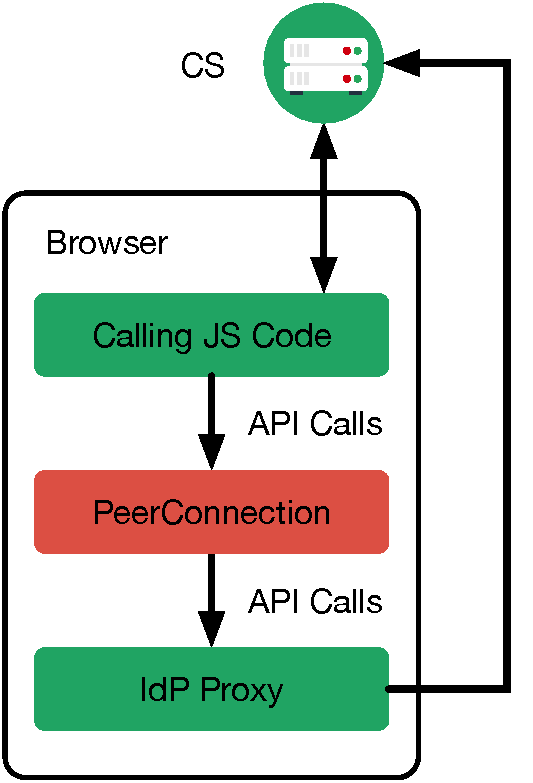
\includegraphics[width=\marginparwidth]{images/localAuthArch}
\caption{Local Authentication Architecture}
\label{fig:localAutharch}
}
Local authentication refers to a scenario where the \gls{cs} also plays the role of the \gls{idp} in the WebRTC identity architecture, as in Figure~\ref{fig:localAutharch}.
It is not the architecture initially envisioned by the specification.
As we explained in Section~\ref{sec:webrtcid}, the decoupling of identity and signalling functions are meant to prevent the \gls{cs} from setting up a man-in-the-middle during the call session establishment.
This architecture may nonetheless be useful.
Firstly, it provides a simple test use case for an \gls{idp} Proxy with a login and password authentication as used by most websites not relying on \gls{idp}.
Secondly, in an interoperable signalling architecture, multiple \gls{cs} are used to establish the session.
A user may not trust the signalling path, except for his own \gls{cs}. 
In this case using his \gls{cs} as an \gls{idp} would offer a protection against man-in-the-middle attack from other \gls{cs}.
Finally, in compatibility scenarios call transit through a legacy interface, for instance, a \gls{sip} Gateway.
In this case, the legacy interface plays the role of both the \gls{cs} and the \gls{idp}.

Functionally, our implementation of the \gls{idp} Proxy maps the identity assertion to the \texttt{contents} parameter, \ie the session fingerprint.
The identity assertion thus serves as the key to retrieve claims covered by the assertion, and verify in the process that these claims were effectively registered on the \gls{idp}.
Figure~\ref{localAuthGen} presents the identity assertion generation interface exposed by the server to the \gls{idp} Proxy and its sequence diagram.
To store a new pair, the \texttt{generateAssertion} function of the \gls{idp} Proxy POST a content to the \texttt{/assertion} REST interface. 
After the server checked that the user is logged in, the user's identity and content parameter are stored in a map and the key is returned with an \gls{http} 200 success response.
The \gls{idp} Proxy then uses the key to instantiate an \texttt{RTCIdentityAssertionResult} (see Figure~\ref{idAssertWebIDL}) and resolve the \texttt{generateAssertion} promise with it.
On the promise's resolution, the browser adds the assertion dictionary to the \gls{sdp} message.

\begin{figure}[H]
\begin{Verbatim}[commandchars=\\\{\}]
dictionary \textcolor{matred}{RTCIdentityAssertionResult} \{
    required \textcolor{matred}{RTCIdentityProviderDetails}       idp;
    required \textcolor{matblue}{DOMString    }        assertion;
\};

dictionary \textcolor{matred}{RTCIdentityProviderDetails} \{
    required \textcolor{matblue}{DOMString    }                domain;
             \textcolor{matblue}{DOMString}                        protocol = "default";
\};

\end{Verbatim}
\caption[RTCIdentityAssertionResult specification in WebIDL]{RTCIdentityAssertionResult specification in WebIDL. The assertion is an "opaque string that MUST contain all information necessary to assert identity". It is consumed by the validating IdP.}
\label{idAssertWebIDL}
\end{figure}

Alternatively, if the user does not have an active session, the \texttt{generateAssertion} promise is rejected with an \texttt{IdPLoginError} \gls{json} object.
This object may contain an \texttt{idpLoginUrl} element, which can be used by the client service to open a login page on the \gls{idp}.
A successful login following this \gls{url} is signalled by a \texttt{LOGINDONE} message sent using the postMessage \gls{api} to the login page's opener window, \ie the communication service client page.

\begin{Verbatim}[commandchars=\\\{\}]
<script>window.opener.postMessage(\textcolor{matblue}{'LOGINDONE'}, \textcolor{matblue}{'*'})</script>
\end{Verbatim}

Figure~\ref{localAuthVerif} shows the \textit{local} identity assertion validation REST interface and its associated sequence diagram.
To validate a received identity assertion, the peer's browser downloads the \gls{idp} Proxy from the \gls{idp} which produced the identity assertion.
The \texttt{RTCIdentityProviderDetails} dictionary (see Figure~\ref{idAssertWebIDL}), included in the assertion, describes the \gls{idp} Proxy location.
Once the browser instantiated the verifying \gls{idp} Proxy, it calls the \gls{idp} Proxy's \texttt{validateAssertion} function.
Our implementation of this function sends a GET request to the \texttt{/assertion} interface, using the provided assertion (see Figure~\ref{idpproxyimplem:getapi}). 
The result of the request is a \gls{json} object containing the stored identity and content.
This object is used to instantiate an \texttt{RTCIdentityValidationResult} dictionary (see Figure~\ref{idValidWebIDL}) which is then returned to the browser.
The browser verifies that the provided \texttt{contents} matches the \gls{sdp} fingerprint attribute, binding the fingerprint to the assertion's \texttt{identity}.

\begin{figure}[H]
\begin{Verbatim}[commandchars=\\\{\}]
dictionary \textcolor{matred}{RTCIdentityValidationResult} \{
    required \textcolor{matblue}{DOMString    }                identity;
    required \textcolor{matblue}{DOMString    }                contents;
\};

\end{Verbatim}
\caption{RTCIdentityValidationResult specification in WebIDL.}
\label{idValidWebIDL}
\end{figure}

\begin{figure*}
\begin{subfigure}{\textwidth}
\begin{center}
    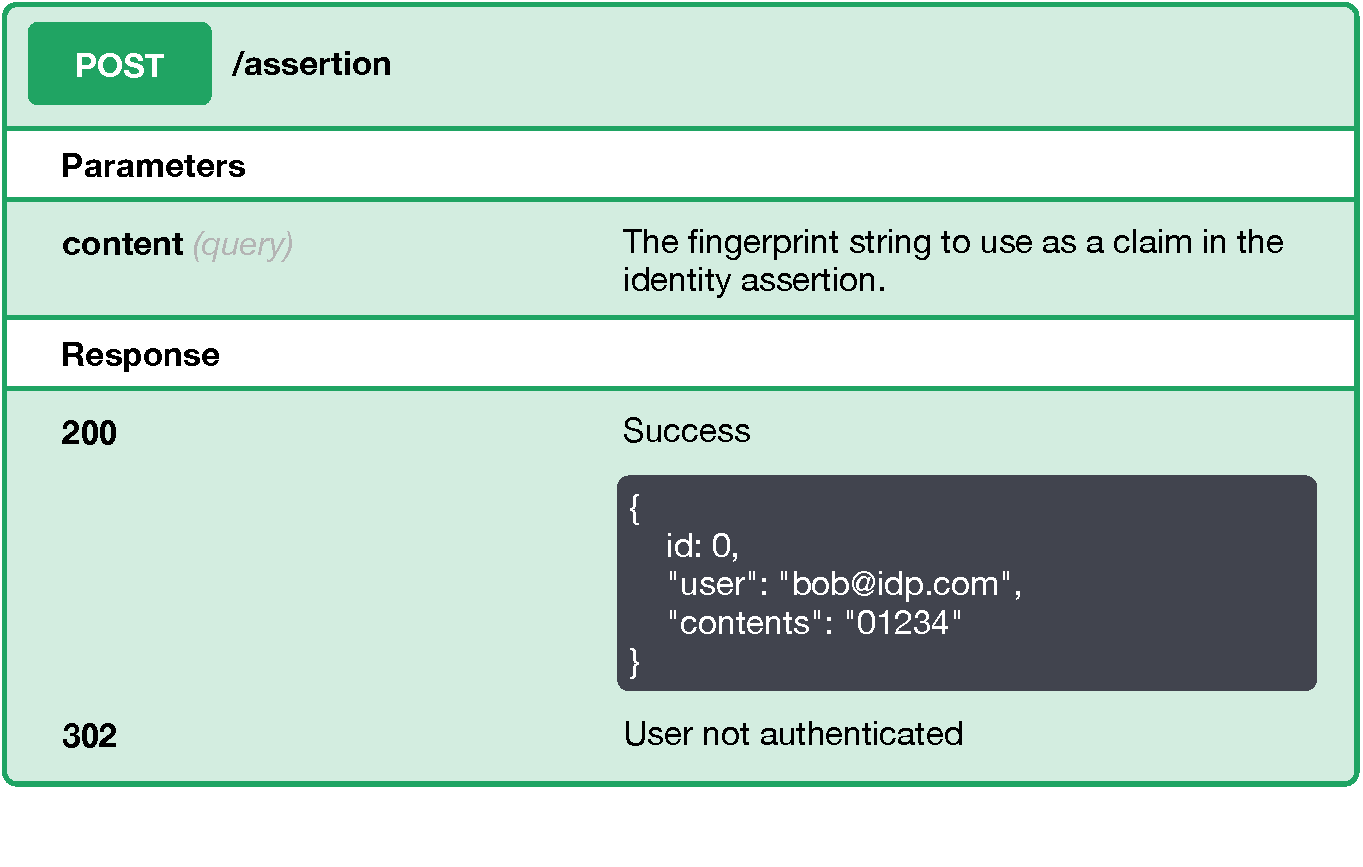
\includegraphics[scale=0.5]{images/localProxyAPIPOST}
\caption{/assertion POST API}
\label{idpproxyimplem:postapi}
\end{center}
\end{subfigure}
\begin{subfigure}{\textwidth}
\begin{center}
    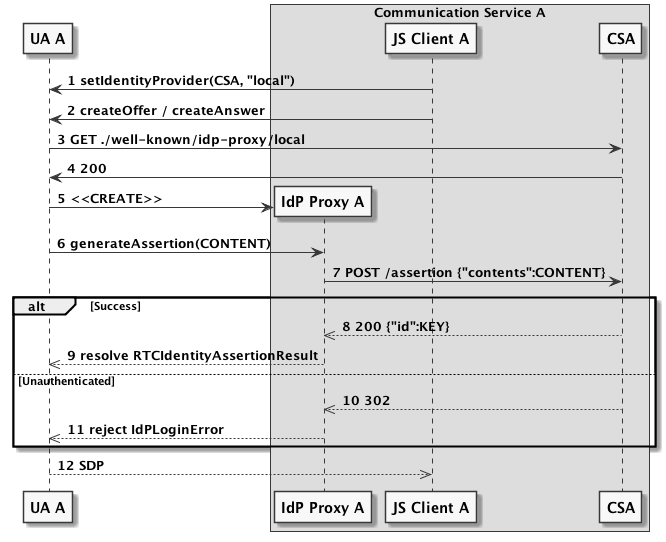
\includegraphics[scale=0.55]{images/localAuthGen}
\caption{Sequence Diagram}
\label{localAuthGen:seq}
\end{center}
\end{subfigure}
\caption{Local Identity Assertion Generation}
\label{localAuthGen}
\end{figure*}

\begin{figure*}[tbp]
\begin{subfigure}{\textwidth}
\begin{center}
    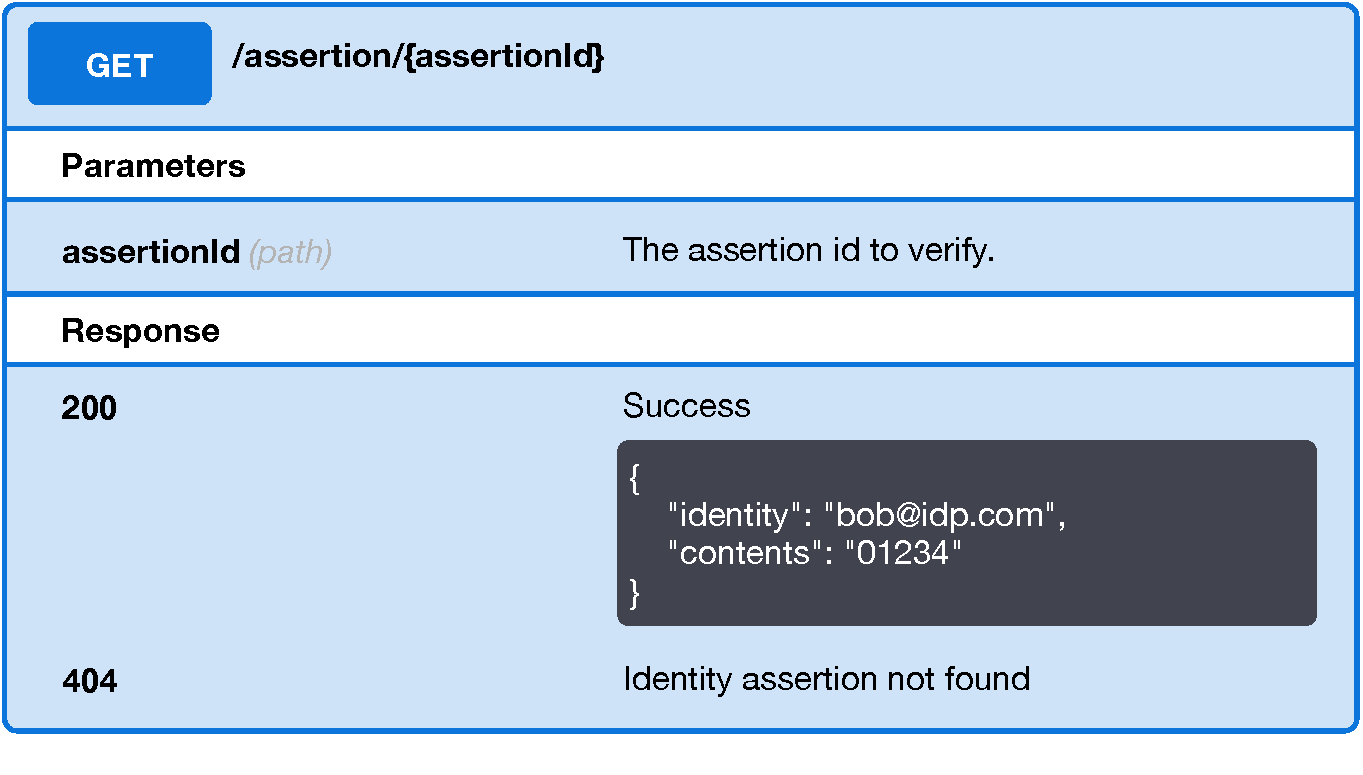
\includegraphics[scale=0.5]{images/localProxyAPIGET}
\caption{/assertion GET API}
\label{idpproxyimplem:getapi}
\end{center}
\end{subfigure}

\begin{subfigure}{\overflowingheadlen}
\centering
    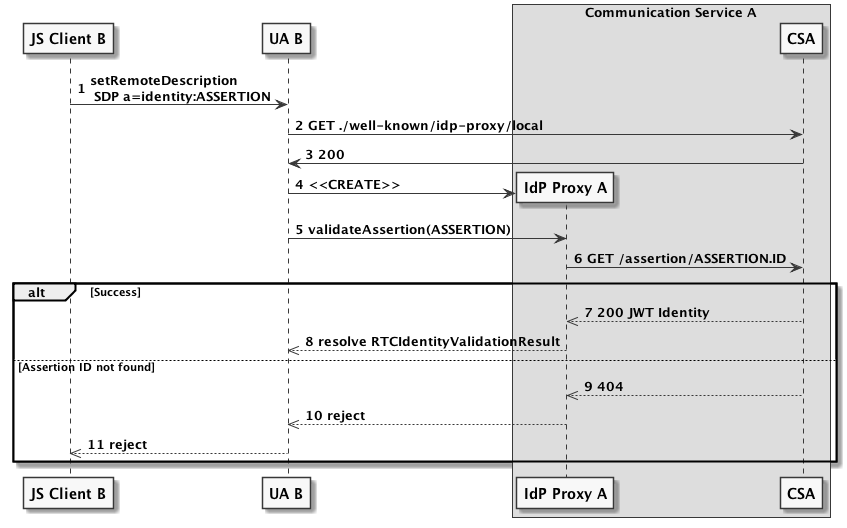
\includegraphics[scale=0.55]{images/localAuthVerif}
\caption{Sequence Diagram}
\label{localAuthVerif:seq}
\end{subfigure}
\caption{Local Identity Assertion Verification}
\label{localAuthVerif}
\end{figure*}


\subsection{IdP Proxy with OpenID Connect}
\label{sec:idpoidc}

In order to integrate our \gls{oidc} servers into the WebRTC identity architecture, the \gls{idp} Proxy acts as the \gls{oidc} client.
In this role, the \gls{idp} Proxy requests an ID Token to the \gls{idp}.
The \gls{idp} authenticates the user and verifies that the user has authorized the \gls{idp} Proxy to obtain an ID Token.
As the \gls{idp} Proxy is a JavaScript code running inside the user's browser, \ie client side rather than server side, we use the \gls{oidc} \textit{implicit flow}.
This flow allows the client to directly get the requested token, as explained in \ref{sec:authProtocol}.
The resulting ID Token covers the user's identity and the session fingerprint as claims.
It thus serves as the WebRTC identity assertion.
Our implementation, however, requires additional modifications to \gls{oidc} requests.

Firstly, we include the session fingerprint as a claim of the ID Token payload so that it is covered by the server's signature.
To send it to the server, we define a new request parameter, \texttt{rtcsdp}, to convey this value in the request.
In practice, this parameter function is quite similar to the \texttt{nonce} request parameter.
Both convey random opaque numbers making the request unique.
However, in some cases, a WebRTC session may reuse a previously established key and thus the same session fingerprint twice.

Secondly, \gls{oidc} interactions with the user normally happen through a new tab or popup opened by the browser.
This graphical user interface allows the \gls{idp} to authenticate the user or request user's consent before authorizing the requesting client.
However, in our case, the \gls{idp} Proxy is running in a sandboxed invisible iframe.
The \gls{oidc} \texttt{/authorize} GET request (see Figure~\ref{idproxyimplem:oidcrequest}) is thus executed through the Fetch \gls{api}\footnote{Fetch is a standard web \gls{api} for network requests similar to the XMLHttpRequest (XHR) interface. An advantage of using the Fetch \gls{api} is that it easily integrates with the promise based WebRTC interfaces. See \url{https://developer.mozilla.org/en/docs/Web/API/Fetch\_API} for more details.}.
Such requests are invisible to the users, no new tab or window are opened.
Hence why the \gls{idp} Proxy has to throw an \texttt{IdPLoginError} in order to interact with the user.
As we described in Section~\ref{sec:idpstd}, this happens if the user is unauthenticated.
In the \gls{oidc} case, it also happens if the \gls{idp} Proxy client has not been authorized by the user.
The login or authorization URL is returned in an \texttt{IdPLoginError} to the \gls{cs}, which opens it so that the user can login or authorize the \gls{idp} Proxy.
In either case, the process followed by the user lands on a page messaging the \texttt{LOGINDONE} signal to the \gls{cs}.
The url of this page is defined using the \texttt{redirect\_uri} parameter of the \texttt{/authorize} request.
When receiving this message, the \gls{cs} restarts the \texttt{generateAssertion} procedure.

Finally, we also implement a new \texttt{response\_mode} value.
In the \gls{oidc} implicit flow, a successful authorization redirects to the client web page.
The ID token would be returned with the redirection either in the redirected URL's query or fragment.
However, both query or fragment are inaccessible from a Fetch (or XHR) response after following a redirection. 
Instead, the \gls{idp} returns the ID Token in the response body.
We thus define a new \texttt{response\_mode} value: \texttt{body} and modify the \gls{idp} server implementation accordingly.

Note that the \texttt{response\_mode} and \texttt{redirect\_uri} parameters are conflicting as they correspond to different HTTP response code, 200 and 302 respectively.
In our implementation, the \texttt{redirect\_uri} is only followed if \texttt{response\_mode} is not set to \texttt{body}.
Figure~\ref{idproxyimplem:oidcrequest} shows our modified \texttt{/authorize} request specification.

\begin{figure*}[tbp]
\begin{subfigure}{\textwidth}
\centering
    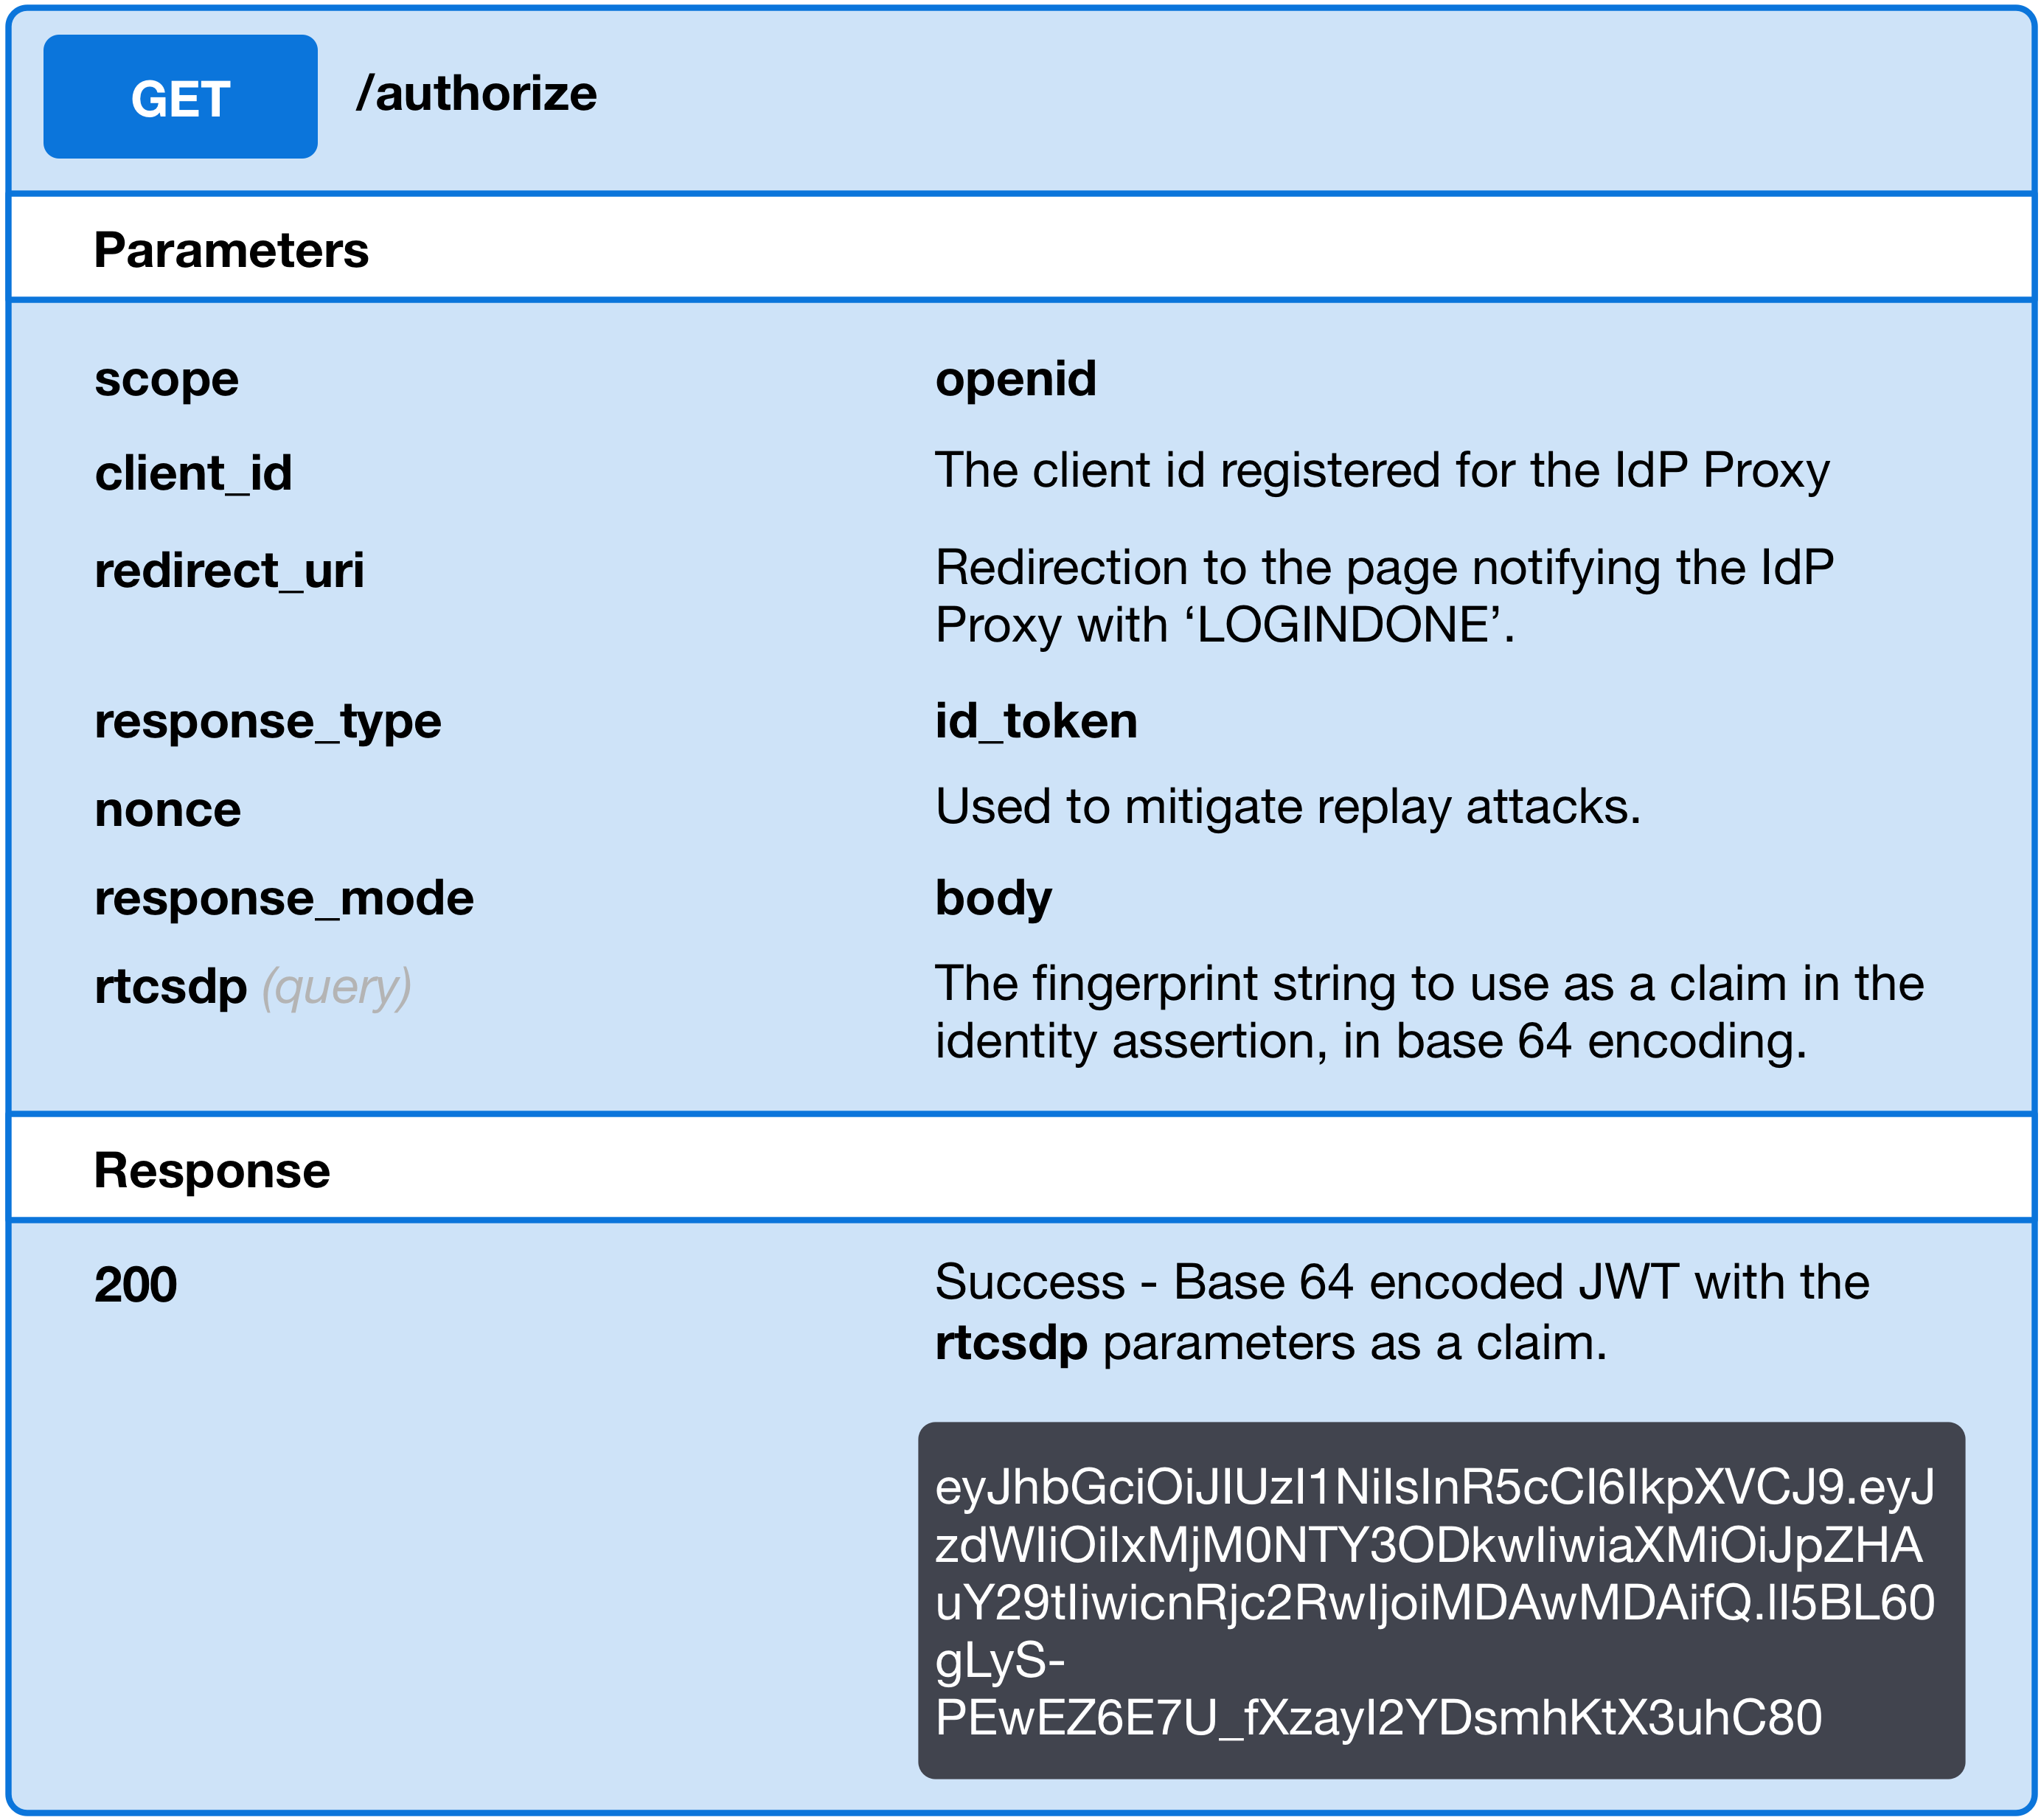
\includegraphics[scale=0.5]{images/OIDCProxyAPI}
\caption{/authorize GET API}
\end{subfigure}

\begin{subfigure}{\overflowingheadlen}
\centering
    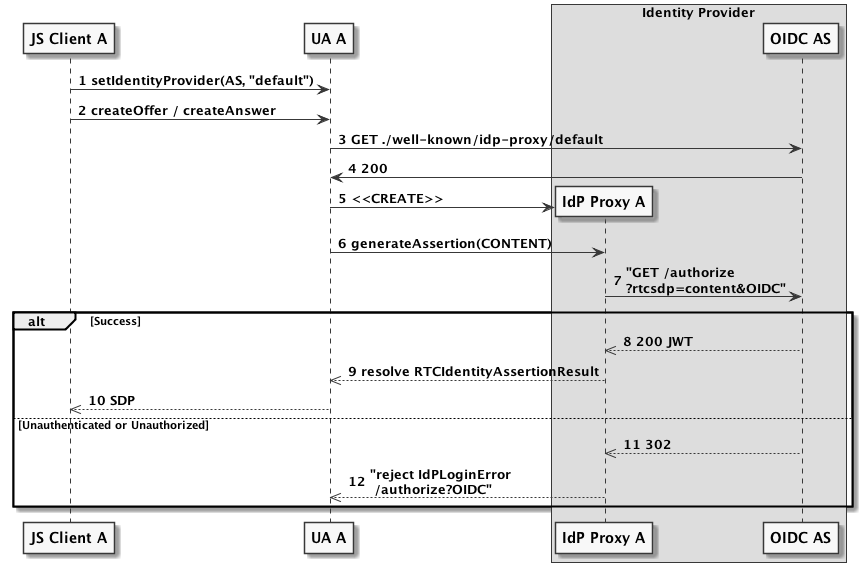
\includegraphics[scale=0.55]{images/oidcAuthGen}
\caption{Sequence Diagram}
\end{subfigure}
\caption{OIDC Assertion Generation}
\label{idproxyimplem:oidcrequest}
\end{figure*}

To verify the ID Token validity, its signature must be verified by the \gls{idp} Proxy when it is executed from the other peer's browser.
It is either possible to add the \gls{idp}'s public key in the \gls{idp} Proxy code or retrieve it from a secured location on the \gls{idp}.
Optionally a reference to the key \gls{url} could be included in the ID Token header \texttt{jku} parameter.
This solution is discouraged by the \gls{oidc} specification which states that ``ID Tokens SHOULD NOT use the JWS or JWE x5u, x5c, jku, or jwk Header Parameter fields''~\cite{sakimura_openid_2014}.


\subsection{Observations}
\label{sec:proxyImplemObs}
We note that the Firefox implementation is more restrictive than the specification regarding identity format.
Firefox requires that the identity, the human-readable identifier, be in an email format with the domain of the email equals to the \gls{idp} Proxy domain.
This format prevents domains from asserting identity from other domains, \eg identifier ending in \url{@orange.com} could not be claimed by an \gls{idp} Proxy from the \url{dr.evil.net} domain.
However, using the email's domain as an indication of the \gls{idp}'s domain name is often an over-simplification.
As an example, Figure~\ref{fig:googleIdSelector} shows the Google identity selection popup.
Although the popup's domain name, \ie Google's \gls{idp} domain, is \url{accounts.google.com}, user's identifiers may end in \url{@gmail.com}.
Some valid identifiers may even end in other domain names if the user did not activate his Gmail mailbox, for example, \url{@orange.com}.

As shown by Table~\ref{tab:localProxyLines} the implementation of the local \gls{idp} Proxy is quite simple.
Proxy, Routes, and Model give the new and total number of JavaScript code lines respectively for the \gls{idp} Proxy, the \gls{http} interface implementation, and the database model.
On the project as a whole, our implementation required only 120 JavaScript code lines.
A number to be compared to the 6641 code lines, excluding NodeJS dependencies, of the full WebRTC service project.

\begin{table}
\begin{tabular}{{@{}lll@{}}}\toprule\toprule
  \textbf{Module} & \textbf{New code lines} & \textbf{Total code lines} \\\midrule
  \textbf{Proxy} & 66 & 66\\
  \textbf{Routes} & 38 & 290\\ 
  \textbf{Model} & 16 & 89\\\midrule
  \textbf{Project} & 120 & 6641\\\bottomrule
  \hline
\end{tabular}
\caption[JS code lines for local IdP Proxy]{JavaScript code lines for the local authentication IdP Proxy implementation.}
\label{tab:localProxyLines}
\end{table}

Compared to the local \gls{idp} Proxy, implementation of an \gls{oidc} \gls{idp} Proxy is a complex task.
Firstly, while following the same structure, the \gls{idp} Proxy is larger due to its requirement of ID Token signature verification, client key retrieval, and the handling of \gls{json} objects.
The \gls{idp} Proxy JavaScript file contains 207 JavaScript code lines.
The more complex modifications are however made on the \gls{oidc} server itself.
We add a few utility functions to the \gls{http} interface, but we also modify the core \gls{oidc} modules to support the parameters we introduced: \texttt{response\_mode=body} and the \texttt{rtcsdp} ID Token claim.
While these modifications are not that heavy in terms of code lines, they require the understanding and modification of a large code base.
As an example, the NodeJS dependency implementing the \gls{oidc} specification contains 1274 code lines in a single file.

Another issue of the \gls{oidc} implementation is its reliance on non-standard modification of the specification.
Industrial deployment of standards protocols may follow strict policies regarding the implementation of non-standard features.
In our case and due to the policies of our company, integrating our proposed change to the \gls{oidc} server in production would have required to first get them published by the OpenID foundation. 
The complexity of the \gls{oidc} implementation does not seem to brings benefits compared to the simple solution of the local authentication \gls{idp} Proxy.

Our implementations shows that \gls{oidc} facilitates the creation and signature of WebRTC identity assertion in an open standard format: \gls{oidc} ID Token.
However, it requires the modification of a complex code base not initially designed for this use case.
While using the ID Token format may have practical use cases to exchange WebRTC Identity assertion.
For some use cases, it may be as simple to use a map interface secured through \gls{https}.

\begin{figure}[h]
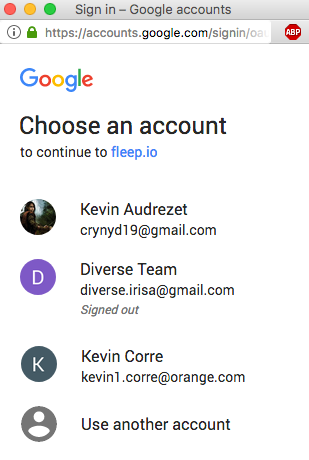
\includegraphics[width=1.3\marginparwidth]{images/googleIdSelector}
\caption[Google Identity Selection Page]{Google identity selection webpage.}
\label{fig:googleIdSelector}
\end{figure}

\section{RQ1.1 Additional Privacy Considerations}
\label{sec:privacyissue}

We presented the WebRTC security architecture in Section~\ref{sec:websecurity} and reviewed previous research works on WebRTC security in Section~\ref{sec:sota2012+}.
From this work, we observed that the identity path proposed by WebRTC security architecture has only been studied from a theoretical point of view and that in these works \gls{idp} had not been considered as possible attackers against the users' privacy.
In this section, we answer RQ1.1 by presenting new risks for the user's privacy introduced by the \gls{idp} Proxy component.
These privacy considerations were revealed by our implementation process.

\subsection{Audience Issue}
In addition to the \texttt{rtcsdp} claim, \ie the session fingerprint, the WebRTC identity assertion carries two important information: the peer's identity in human readable form, and the peer's identity provider fully qualified domain name.
Both pieces of information are necessary so that the assertion can be verified and associated with a peer's identity.
But from a privacy point of view, they are sensible identifying information.
In the \gls{sdp} message, the identity assertion is an opaque string encoded in base 64, which means that it has no actual definition.
However, the \gls{idp} Proxy can be downloaded by any party and instantiated to decode the identity assertion.

Although we explain this privacy issue with the \gls{oidc} scenario, it is present whether or not the \gls{idp} Proxy is based on \gls{oidc}.
As we explained in Section~\ref{sec:authProtocol}, OpenID Connect is based on OAuth2, an authorization protocol.
As such the concept of authorization and user consent is central to the protocol.
In theory, the client, identified by the \texttt{client\_id} in \gls{oidc} requests and the \texttt{audience} claim, is authenticated by the \gls{idp}.
In the implicit flow, the client authentication is not performed explicitly and instead relies on the \texttt{redirect\_uri} redirection to the client.
In the WebRTC use case of user-to-user authentication, the \texttt{redirect\_uri} is not followed as the ID Token is transmitted to the other peer over \gls{sdp} signalling.
There is no clear definition of the intended audience\footnote{The audience may not even be known a priori, for instance in the case of a call to an anonymous peer.} and in our implementation we define and use a unique \gls{idp} Proxy client and \texttt{client\_id}.
We explored the alternatives of one \texttt{client\_id} for each users, each \gls{cs}, or for each pair of user/\gls{cs} without finding clear advantage to any of these solutions.

As represented in Figure~\ref{idProxyWebIDL}, both \texttt{generateAssertion} and \texttt{validateAssertion} functions use an origin parameter.
This parameter is the origin of the \gls{cs} which required the instantiation of the \gls{idp} Proxy
However, the \texttt{validateAssertion} is executed after the identity assertion is transmitted over the signalling path.
As a result, the \gls{idp} does not know the signalling endpoint's origin during the generation of the assertion.
Some policy checks could still be applied during the execution of the \texttt{validateAssertion} function, eventually preventing the decoding and decryption of the identity assertion.
But the specification does not define the error that should be returned in this scenario and does not plan for transmitting a consent request back to the user.
Implementing such consent mechanism could be allowed using a push notification to the user's device.

On the other hand the \texttt{generateAssertion} can interact with the user through the \texttt{\gls{idp}LoginError}.
It can thus be subject to user authorization and \gls{idp} policies, as long as the \gls{idp} implements such mechanism.
Otherwise, without appropriate protection on the \gls{idp} Proxy, a web page could look for the user's identity.
This could reveal user identities, or at least existing user accounts on \gls{idp}s.
For instance, given a list of WebRTC compatible \gls{idp}s, running the script described in Figure~\ref{fig:audAttack} would reveal identity assertion from unprotected \gls{idp}s with active sessions.
This is a major issue, and implementors should take appropriate measures to protect their interfaces against such vulnerabilities.

\begin{figure}[H]
\begin{Verbatim}[commandchars=\\\{\}]
\textcolor{matred}{IdPArray}.\textcolor{matblue}{forEach}(function(idp)\{
    var \textcolor{matred}{pc} = new RTCPeerConnection()
    \textcolor{matred}{pc}.\textcolor{matblue}{setIdentityProvider}(idp.domain, idp.proxy)
    \textcolor{matred}{pc}.\textcolor{matblue}{getIdentityAssertion}()
    .\textcolor{matblue}{then}(res => {\textcolor{matblue}{alert}("Got your ID token: "+res)})
\})
\end{Verbatim}
\caption[JS Code for WebRTC Identity Collection]{This JavaScript code starts multiple invisible WebRTC sessions. It then associates an \gls{idp} for each of them and extract their generated identity assertion. }
\label{fig:audAttack}
\end{figure}

The only visible hint to the user that a WebRTC session is starting happens when the browser request consent to share video and audio input.
But it is also possible to start a WebRTC session without any attached media, as in our example in Figure~\ref{fig:audAttack}. 
In this case, the session is invisible for the user without looking into the browser WebRTC session statistics.
The \gls{ice} IP leak issue (see Section~\ref{sec:sota2012+}) is due to the same weakness where the user may not see and control the start of a WebRTC session.
A solution implemented to fix this issue is to tie the implicit sharing of private \gls{ip} addresses with the explicit authorization granted to the \texttt{getUserMedia} interface~\cite{I-D.ietf-rtcweb-ip-handling}.
The same solution could work to implicitly authorize the sharing of identity information for legitimate WebRTC session.
However, it may prove too restrictive for some use cases such as authenticated data sessions.
An alternative solution would be to have the browser explicitly manage consent for authentication.

\subsection{IdP in a Central Position}
\label{sec:idptrack}
The WebRTC Identity Architecture replaces the users' trust in \gls{cs} by trust in \gls{idp} to ensure secure communication through untrusted signalling.
Although \gls{idp} already occupy a central role on the Web, they gain the ability to track any user call covered by an identity assertion.

Indeed, the \gls{idp} Proxy code is deployed on both sides of the call and running in the context of its \gls{idp}'s origin.
It is also subject to the same sandbox restrictions whether on the identity assertion generation or validation side.
This implies that an \gls{idp} Proxy can place and read cookies on a user's \gls{ua} verifying an assertion.
Note that the user verifying the identity assertion does not actively access the \gls{idp}, it only receives a call offer or answer containing an identity automatically verified by the browser.
The \gls{idp} Proxy reading cookies could allow the \gls{idp} to track a user's call history.
Eventually, even an identity unknown to the \gls{idp} could be linked with a known identity, and the call history versed into an existing profile.
The \gls{idp} can also track user calls across multiple \gls{cs}, as long as they use, or are called with the same \gls{idp}. 

%\todo{If there is time, write some line of code to write in local storage from verifyAssertion function}

Reusing the classification proposed by Vapen et al., presented in Section~\ref{sec:vapen}, this ability to track user call history could at least be classified as \textit{R+}.
It could even be classified as \textit{R++}, the highest privacy risk level, with regards to the verifying user's data as it would fall under the \textit{Friend's data} class of privacy risk.
However, users may not have authorized or even be aware of such tracking capacity.
It is interesting to note that the information sharing relation is here reversed between the \gls{idp} and the \gls{cs}.
In a classical authentication delegation, the user authorizes the \gls{idp} to share resources with the \gls{rp}.
However, in this case, the \gls{cs} is in possession of call information and shares them with the \gls{idp} by adding it to the call setup.

\section{Why Can't Users Choose their Identity Providers on the Web?}
\label{userschooseidp}
In Section~\ref{sec:privacyissue}, we presented how the WebRTC identity architecture may be used by \gls{idp} to track user calls without explicit user's authorization or awareness. 
%What we call \textit{identity continuity} implies that the \gls{idp} set by the \gls{cs} for the communication session would be the same as the one the user would have previously chosen to authenticate to the CS\footnote{In the scenario of the WebRTC identity architecture, a peer is presented with two identities. One identity displayed on the \gls{cs} user interface, and the other validated by an \gls{idp} proxy and displayed by the peer's browser. For a coherent user experience both identities should ultimately be the same and thus have the same \gls{idp}.}.
As shown by Vapen~\etal\cite{DBLP:conf/sec/VapenCMS15}, on the web, users are presented with a very limited choice of \gls{idp} when signing in with authentication delegation.
They reported that 47\% of observed \gls{rp} offer only one \gls{idp}, and only 19\% offer four or more \gls{idp}.
Due to the identity continuity constraint\footnote{We presented the identity continuity constraint in Section~\ref{sec:websecurity} which implies that the \gls{idp} set by the \gls{cs} for the communication session would be the same as the one the user would have previously chosen to authenticate to the CS.} the same limitation on offered \gls{idp} choices applies to WebRTC \gls{idp}.
Users may have more trust in \gls{idp} whose business model does not rely on selling personal data or which they would host themselves~\cite{sporny2011webid}.
However, current \gls{sso} implementations do not permit users to make this choice.

Several reasons could explain that users choice is limited by the decision of the \gls{cs}.
Verifying the validity of these reasons would reveal if ``we can let users chose actors they trust to participate in the communication setup'' (RQ3) and eventual solutions to achieve this.
In this study we thus address the following questions:
\begin{itemize}
\item \textbf{RQ3.1}: Do \gls{rp} require specialised \gls{api}?
\item \textbf{RQ3.2}: Is dynamic discovery and registration commonly available for \gls{rp}?
\item \textbf{RQ3.3}: Do \gls{rp} requires a trust relationship with the supported \gls{idp}?
\end{itemize}


\subsection{The Study: OAuth Request Collection}
\label{userschooseidp.study}
To answer the first of our research questions we implement a browser extension to parse the browser navigation history and look for OAuth~2 and \gls{oidc} authorization request \gls{url}.
These requests can be identified as OAuth~2 requests by observing the presence of keyword parameters.
They contain information identifying the \gls{rp} making the request, the \gls{idp} to which the request is destined and the scopes requested by the \gls{rp}.

\begin{figure}[H]
\begin{Verbatim}[commandchars=\\\{\}]
\textcolor{matred}{https://accounts.google.com/o/oauth2/auth}?
     \textcolor{matblue}{client_id}=74[...].googleusercontent.com&
     \textcolor{matblue}{response_type}=code&
     \textcolor{matblue}{redirect_uri}=http://www.dailymail.co.uk/
     registration/signin/google.html&
     \textcolor{matblue}{scope}=email+https://www.googleapis.com/
     auth/plus.login&
     [...]
\end{Verbatim}
\caption{Example of an OAuth~2 request collected by our extension.}
\label{fig:oauth2req}
\end{figure}

The \gls{url} in Figure~\ref{fig:oauth2req} is an OAuth~2 request for an \texttt{accounts.google.com} (URL Domain Name) authorization following the OAuth~2 code flow (\texttt{response\_type=code}).
The request comes from the OAuth~2 client \texttt{74658[...].apps.googleusercontent.com}, also identifiable through the \texttt{redirect\_uri} parameter as \texttt{dailymail.co.uk}.
Comparison of redirection \gls{uri} domains allows associating client from several \gls{idp} to a single actual \gls{rp}.
For instance, this client and the \texttt{facebook.com} client registered as \texttt{146[...]95} both share the same \texttt{redirect\_uri} domain name.
The requested scopes are \texttt{email} and \texttt{\url{https://www.googleapis.com/auth/plus.login}}.
Note that these \gls{url} do not contain private information regarding the user as they are accessed before the user is identified or authenticated.

%We submitted our extension to a panel of thirty computer scientists from our laboratory.
%After installing the extension and being presented with an explanation of the study and a short disclaimer, they had to click on a button to actually launch the data collection and submit the results. 
% Of the thirty participants, about half submitted actual results. As it appeared, the others avoided to use \gls{sso} solutions and their instance of the extension did not found OAuth~2 requests.

To collect data, we manually visit each of the top 500 websites from the Alexa ranking\footnote{\url{http://www.alexa.com/topsites}} and try to use each one of the \gls{sso} solutions offered by these websites\footnote{Our initial objective was to share the extension to a large panel. We later switched to the Alexa ranking as our panel was too small. However, a large-scale study could deliver interesting results, particularly regarding smaller websites.}.
The visited \gls{url} are recorded into the browser history and then parsed by our extension.
In Section~\ref{userschooseidp:h1} we present the results of our study and use them to answer RQ3.1. 
Finally, we use data on collected \gls{rp} and \gls{idp} to answer RQ3.2 and RQ3.3 in Sections~\ref{userschooseidp:h2}~and~\ref{userschooseidp:h3} respectively.

As our data-collection search is focused on OAuth~2, we do not collect requests for \gls{idp} using other protocols, \eg Twitter and Amazon.
However, we scarcely encounter \gls{rp} offering only these \gls{idp}, as a result, the large majority of visited \gls{rp} is captured by our extension.
In total, we observe 103 unique \gls{rp} and 23 OAuth~2 provider's domain names. 
The two biggest observed \gls{idp}s are undoubtedly Facebook and Google, respectively serving 63 and 52 \gls{rp}.
The third most observed \gls{idp} is Twitter with 30 request \gls{url}, but it uses OAuth~1 and as such is not included in our data.

While our results confirm the claim that users are offered a limited choice of \gls{idp}, interestingly we also observe some variations of the number and domain of supported \gls{idp} based on \gls{rp} geographical origins.
Firstly, Chinese websites only offer to log in through Chinese \gls{idp} such as QQ.com\footnote{Chinese \gls{idp} also vary by the type of authentication mechanism as they often use phone authentication through a QR code.}. 
Occidental websites, \ie North-American and European, mostly offer to log in through one or both of the top two \gls{idp}, sometimes with a third solution.
Finally, Russian websites offer the largest number of solutions as they include Russian \gls{idp}, \eg VK.com, and occidental \gls{idp} often not limited to the top three providers.
Other regions were not represented in sufficient numbers to draw any conclusion.


\subsection{RQ3.1: Do RP require specialised API?}
\label{userschooseidp:h1}
\gls{rp} not only require user authentication but also authorization to access protected resources.
These resources may vary in nature, and may not share a standardised data format when of the same type.
One reason for \gls{rp} not to allow signing in with any \gls{idp} could be that they require specific resources, which are not available on any \gls{idp}.

We classify \gls{rp} in three categories: \textit{Authentication}, \textit{Profile}, and \textit{Specialised}, in function of the scope observed in OAuth~2 authorization requests.
Authentication classed \gls{rp} only require an assertion that the user got authenticated by the \gls{idp}.
Any \gls{idp} could serve such \gls{rp}, given a standardised assertion (\eg a signed \gls{jwt}).
This authentication assertion may also contain the user identifier for the \gls{rp}'s use.
\gls{rp} classified as Profile require basic user profile information in addition to an authentication assertion.
These pieces of information are often used to complete their own database and provide a personalised user experience.
\gls{idp} would need to give access to resources in a standardised data format in order to avoid a specific implementation on \gls{rp} side.
Finally, Specialised \gls{rp} require specific resources, for instance, write access on a user shared repository.
By definition, services provided by \gls{rp} of this class are specialised to use resources from a few \gls{idp}, each one requiring its own implementation.
They cannot be generalised to cover a broad range of \gls{idp}.

Figure~\ref{fig_rpclass} presents these classes, ordered by specificity. 
Indeed, access to a particular \gls{api} is more specific than accessing generic profile information.
Similarly, getting access to a username and phone number is more specific than authentication, which could be abstracted to a boolean, \ie authenticated or not.
Although special cases may exist, \eg access to authorized resources without authentication of the user, this classification allows us to define which \gls{rp} could, in theory, accept any \gls{idp}, and which one would be bound to a particular \gls{api}.

\begin{figure}

\begin{center}
    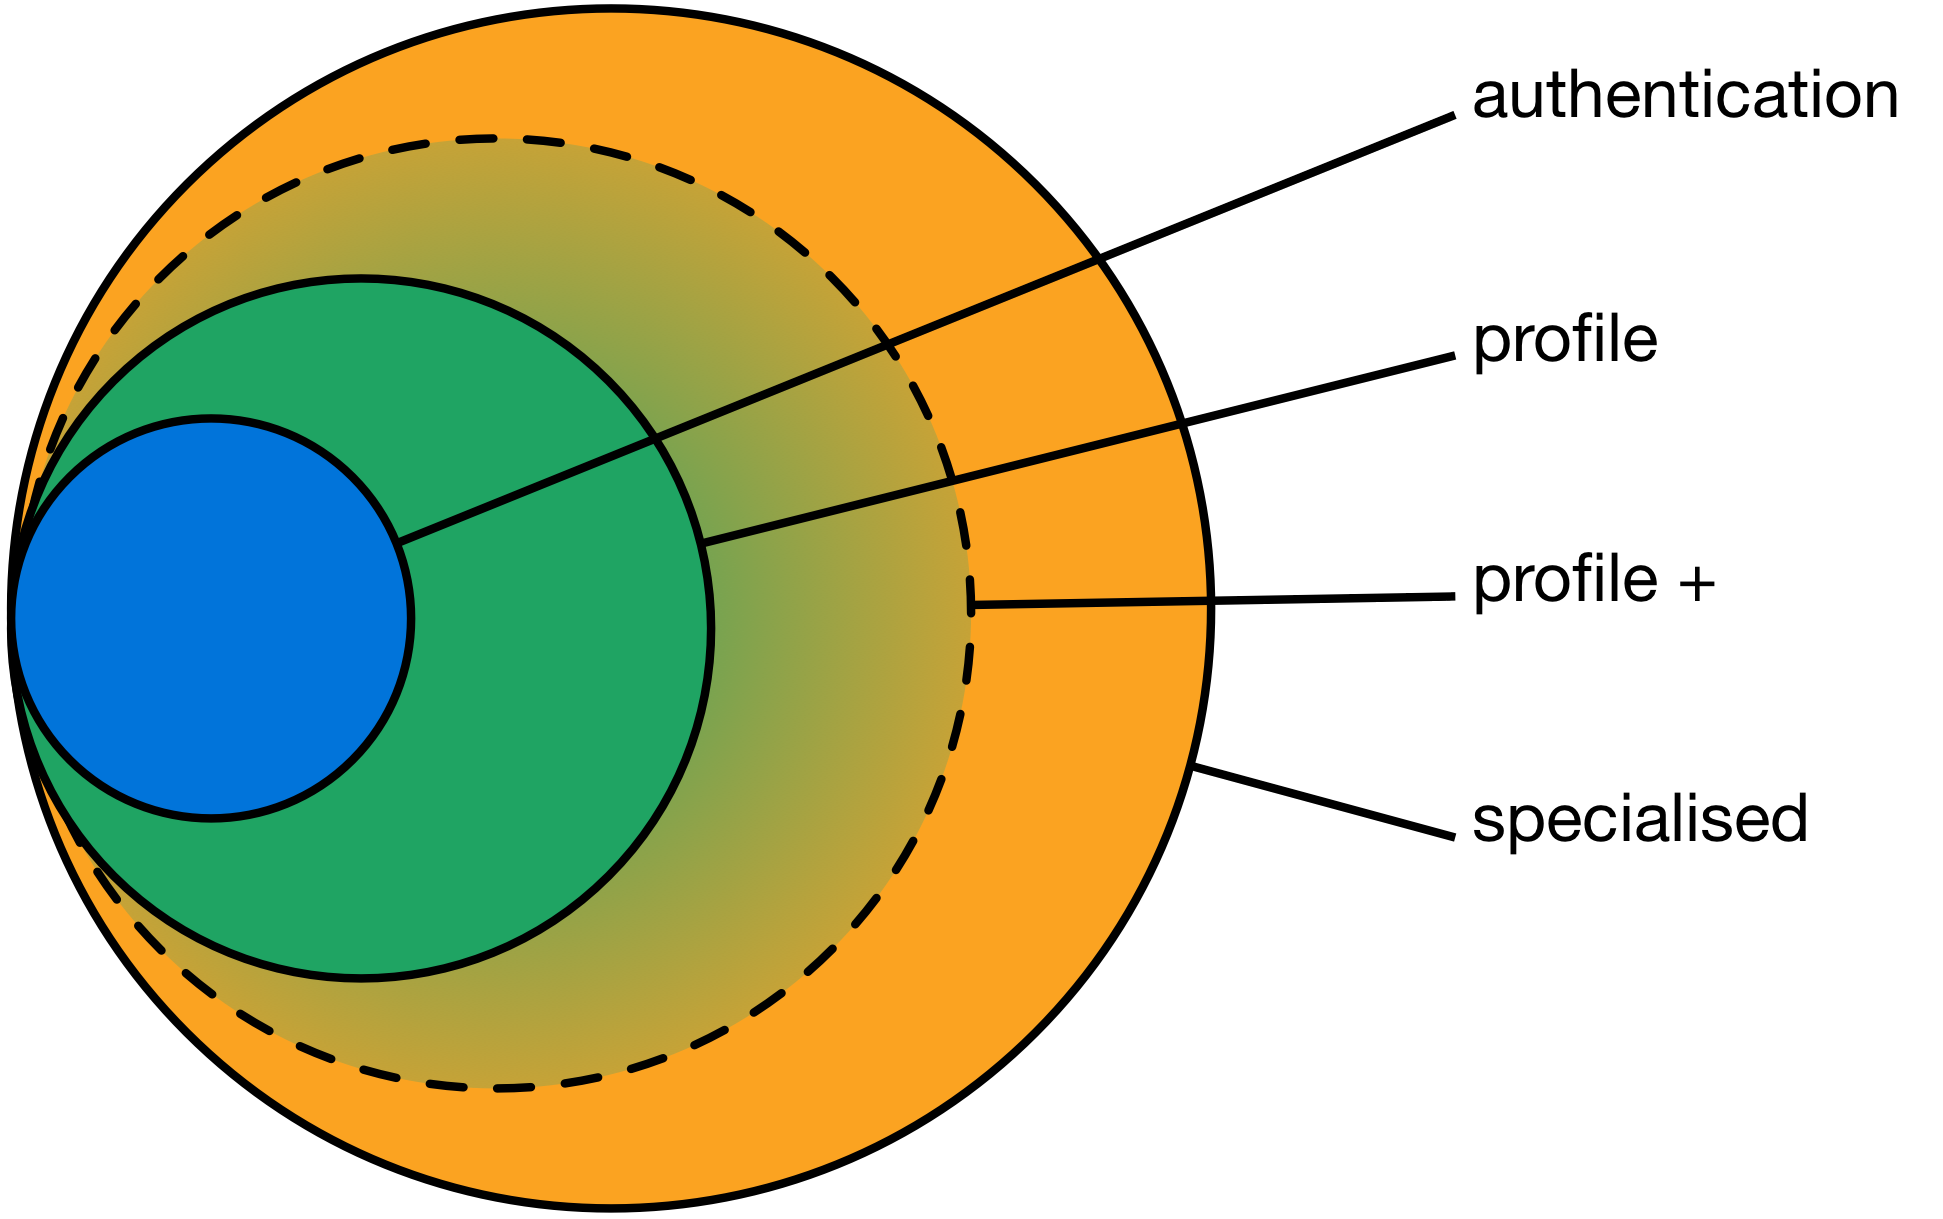
\includegraphics[scale=0.5]{images/authClasses2}
%\begin{tikzpicture}[scale=.9, transform shape]
%\draw(0,0) circle (0.5cm);
%\draw(0.5,0) circle (1cm);
%\draw [dashed] (1,0) circle (1.5cm);
%\draw(1.5,0) circle (2cm);
%
%\draw (0,0.5) -- (4,2);
%\draw (1.5,0) -- (4,1);
%\draw (2.4,-.5) -- (4,0);
%\draw (2.8,-1.5) -- (4,-1);
%
%\node [anchor=west] at (4.2,2) {authentication};
%\node [anchor=west] at (4.2,1) {profile};
%\node [anchor=west] at (4.2,0) {profile+};
%\node [anchor=west] at (4.2,-1) {specialized};
%
%\end{tikzpicture}
\caption{Classification of RP-IdP relationships.}
\label{fig_rpclass}
\end{center}
\end{figure}

We classify each \gls{rp}-\gls{idp} relationships, \ie each collected \texttt{client\_id}, into one of our three classes.
We evaluate from the available documentation if the requested scopes give access to a specialised \gls{api}, a profile information \gls{api}, or an authentication assertion.
Differences between classes may be blurry, for instance, email and friends list can be considered as user profile information.
However, email alone is often used as a unique user identifier in conjunction with a proof of authentication.
\gls{oidc} defines a list of user-information claims and their types, we consider this as the standard for user information.
Other types of information and \gls{api}, \eg friends lists or cloud access, are non-standard and not available from every \gls{idp}.
We classify these requests outside of the Profile and Authentication classes as Specialised.
Ultimately we define our classes as follows:

\begin{itemize}
\item \textbf{Authentication:} requests only subscriber identifier scopes, \eg the \texttt{openid} or \texttt{email} scopes.
\item \textbf{Profile:} requests scopes for user informations equivalent to \gls{oidc}'s standard claims.
\item \textbf{Specialised:} requests any scope not classified as either Authentication or Profile.
\end{itemize}

Some \gls{rp} offer to sign in with multiple \gls{idp} and may require different types of information for each \gls{idp}.
As a result, they may be classified differently for each of their implemented \gls{idp}.
Based on common \texttt{redirect\_uri} domain names, we regroup clients into unique \gls{rp}. 
For each \gls{rp} we attribute a minimum (MIN) and a maximum (MAX) classes, noted MIN/MAX.
As an example, a \gls{rp} classified as Authentication/Profile requires to access profile information on some of the supported \gls{idp} options, but only requires an authentication proof and a unique identifier on at least one offered \gls{idp}.
\gls{rp} offering only a single \gls{idp} are classified as MIN/-.

\subsubsection{Result analysis}
Our observations, summarised in Table~\ref{tab_class}, reveals that a majority of \gls{rp}, \SI{58}{\percent} of 103, are classified as Authentication or Profile. 
MAX-classed \gls{rp}, \SI{40}{\percent} in total, are the one providing support for multiple \gls{idp}.
In our observations, 24 out of 56 \gls{rp} with a Specialised class are classified with a MIN class of Authentication or Profile.
This double classification demonstrates that while some websites require Specialised services, they also adapt to support other \gls{idp} offering fewer resources.
Note that this also leads to different privacy risk level for the user.
On the other hand, \SI{34}{\percent} of observed \gls{rp} are rated as MIN-Specialized.

The large majority of Specialised \gls{rp} use resources from \gls{osn} such as friends list, user likes, and extended profile information.
While data from different social networks can be similar from a conceptual point-of-view, the format and \gls{api} used to access these data depend on the functionalities and concepts offered by social networks.
In these cases, the user fully depends on implementation choices by \gls{rp}.
Although being a standard protocol, OAuth~2 lets \gls{idp} define their scopes and data formats.
As a result, \gls{idp} may provide similar results in different scopes and data formats.
For instance, we observed six different scopes for email access and seven different scopes for basic profile information.
This gives an indication on the lower bound of the implementation work that \gls{rp} must complete to support these \gls{idp}s. 

\begin{table}
\centering
\begin{tabular}{@{}lcc@{}}\toprule\toprule
  \textbf{Min/Max Classes} & \textbf{Observed} & \textbf{Risk class}\\\midrule
  \textbf{Authentication/-} & 10\% (10) & $R-$\\
  \textbf{Authentication/Auth} & 1\% (1) & $R-$\\
  \textbf{Authentication/Profile} & 9\% (9) & $R-$\\
  \textbf{Authentication/Special} & 6\% (6) & $[R-;RA+]$\\\midrule
  \textbf{Profile/-} & 13\% (13) & $R-$\\
  \textbf{Profile/Profile} & 2\% (2) & $R-$\\
  \textbf{Profile/Special} & 17\% (18) &$[R-;RA+]$\\\midrule
  \textbf{Specialised/-} & 26\% (27) & $[R; RA+]$\\
  \textbf{Specialised/Special} & 5\% (5) & $[R; RA+]$\\\midrule
  \textbf{No Scope} & 11\% (11) & \\
  \textbf{Total} & 100\% (102) & \\\bottomrule
  \hline
\end{tabular}

\caption[Observed Relying Parties' Classes]{Observed relying parties' classes\\ Some RP offer to sign in with a single IdP, we classify them with a single class, \eg Profile/-. 
Other RP offer multiples IdP, their relations with these IdP may belong to a single class, \eg Profile/Profile, or different classes, \eg Auth/Special.
For these RP we show the minimum and maximum classes they offer.
Risk class refer to privacy risk classes as defined by Vapen et al. (see Section~\ref{sec:vapen}).
When a RP has different risk class due to multiples RP-IdP relationships, we give an interval for the Risk classification. }
\label{tab_class}
\end{table}

\gls{oidc} solves this problem by standardising basic profile claims (\eg profile, email, address, ...) as well as the scopes, endpoint, and data format to retrieve these pieces of information.
From our observation, only four \gls{idp} out of twenty where implementing \gls{oidc}, as reported on Table \ref{tab_discoveryimplem}.
Notably, Google is one of the OIDC providers and serves \SI{50}{\percent} of observed \gls{rp}, while Facebook does not implement it and serves \SI{63}{\percent} of observed \gls{rp}.
Other \gls{idp} serve less than \SI{6}{\percent} of \gls{rp} each.
However, out of the 52 \gls{rp} using Google's \gls{sso}, only 22 request standard \gls{oidc} scopes, and from these 22 only 10 request \gls{oidc} ID Token.
Surprisingly, we also observe that out of the 34 \gls{rp} using the Google \gls{api} scopes, 19 were using deprecated scopes.

\gls{rp} of MIN-Authentication and MIN-Profile classes represent \SI{58}{\percent} of all observed \gls{rp}. 
We defined these classes as being equivalent to claims covered by \gls{oidc} requests.
It appears that from our observations, the quantity and type of information shared under these scopes would be sufficient to login into a majority of websites.
We thus conclude that current standards for \gls{api} and data format do not appear to be a hindrance to \gls{sso} interoperability.
However, there is a clear lack of implementation of these standards from big \gls{idp}, \eg Facebook not implementing \gls{oidc} or Twitter not implementing OAuth~2.
But the lack of implementation effort also comes from \gls{rp}.
A non-negligible proportion of them did not update their \gls{sso} implementations to the latest versions.
Implementation cost may be a reason, but we also note that studied websites come from the most 500 visited websites.
They should have the resources to update their implementations.

Regarding scopes for sharing \gls{osn} data such as friends list, we observe that 43\% of \gls{rp} using \gls{osn} data also implemented other \gls{idp} without requesting \gls{osn} data.
This is even the case when such data would be available from the \gls{idp}, \eg with the \texttt{accounts.google.com} \gls{api}.
On one hand, a standard format for \gls{osn} data could allow more interoperability between \gls{rp} and \gls{osn} based \gls{idp}.
But on the other hand, since the \gls{rp} can accept non-\gls{osn} \gls{idp}, sharing of \gls{osn} data appears to be non-mandatory.
The possibility to opt-out of consent for data sharing is however often not offered or not clearly advertised.

\subsection{RQ3.2: Is dynamic discovery and registration commonly available for RP?}
\label{userschooseidp:h2}
In order to support sign-in on an \gls{rp} with any \gls{idp}, the identity protocol must offer discovery mechanism. 
This mechanism allows the \gls{rp} to find the \gls{idp}'s protocol parameters from a \gls{uri} provided by the user. 
Depending on the protocol this \gls{uri} may be for instance the user identifier or a resource location on the \gls{idp}. 
Without discovery, the \gls{rp} may not know which endpoint to use on the \gls{idp}, or which public keys and algorithms to use to verify information provided by the user or the \gls{idp}.
Additionally, the protocol should also allow interactions between \gls{idp} and \gls{rp} without prior manual configuration.
Some protocols require the \gls{rp} to possess credentials to be authenticated by the \gls{idp}.
In this case, a dynamic registration process must take place before any further interactions.

For instance, OAuth~2 recommends that the \gls{rp} possesses a client identifier and secret for authentication in order to retrieve an access token.
The use of an unregistered client is not excluded by the specification, but our investigation did not reveal any use of this. 
Similarly, \gls{oidc} requires the \gls{rp} to be authenticated to get access and identity tokens. 
The current OAuth~2 version does not specify dynamic registration mechanism, but \gls{oidc} optionally offers discovery~\cite{sakimura_openid_discovery} and dynamic registration~\cite{sakimura_openid_dynreg}.
\gls{oidc} discovery uses Web Finger~\cite{RFC7033} to find user's \gls{idp} from the user identifier and standardises \gls{idp}'s metadata location.
Metadata are in turn used to find, if available, the dynamic registration endpoint. 
However, both discovery and dynamic registration extensions are optional.
\gls{rfc}~7591~\cite{RFC7591} proposes to generalise the specifications of \gls{oidc} discovery and dynamic registration to the broader OAuth~2 specification.

\begin{table}
\centering
\begin{tabular}{@{}lccc@{}}
  \toprule\toprule
  \textbf{IdP} & \textbf{RP} & \textbf{OIDC} & \textbf{Metadata}\\
  \midrule
  www.facebook.com     & 63 & $\times$ & $\times$ \\
  accounts.google.com      & 52  & $\checkmark$ & $\checkmark$ \\
  oauth.vk.com          &6 & $\times$ &  $\times$ \\
  graph.qq.com          &5 & $\times$ &  $\times$ \\
  login.live.com          & 3 & $\times$ & $\checkmark$ \\
  account.live.com          &3 & $\times$ & $\times$ \\
  www.linkedin.com          &3 & $\times$  & $\times$ \\
  connect.ok.ru          &3 & $\times$ &  $\times$ \\
  login.microsoftonline.com &1 & $\checkmark$ & $\times$ \\
  services.Adobe.com     &1 & $\checkmark$ & $\times$ \\
  github.com              &1 & $\times$  & $\times$ \\
  feedly.com             &1 & $\times$ &  $\times$ \\
  www.livejournal.com      &1 & $\times$ &  $\times$ \\
  connect.mail.ru          &1 & $\times$ &  $\times$ \\
  open.weixin.qq.com      &1 & $\times$ & $\times$ \\
  api.weibo.cn            &1 & $\times$ & $\times$ \\
  mixi.jp                  &1 & $\checkmark$ & $\times$ \\
  oauth.riotgames.co         &1 & $\checkmark$ & $\times$ \\
  \midrule
  \textbf{Total}                & 103 & 5 & 3 \\
  \bottomrule
\end{tabular}

\caption{Observed OIDC and discovery features Implementations}
\label{tab_discoveryimplem}
\end{table}

Table~\ref{tab_discoveryimplem}, summarizes the observed OAuth~2 \gls{idp}.
In total, we collect 23 unique \gls{idp} domain names.
Out of those, 15 are not requested with a scope parameter and are not included in our OIDC features investigation.
For instance, the \url{rambler.ru} request to \url{instagram.com} does not contain a scope parameter, but Instagram still asks some authorization to the user.
On the other 18 unique \gls{idp} domain names, only 5 are used with a \texttt{openid} scope.
This indicates implementation of \gls{oidc}.

The standard end-point for \gls{oidc} configuration metadata is accessed on the path \texttt{/.well-known/openid-configuration}.
We access metadata for each observed \gls{oidc} provider.
In total, only two out of five offer \texttt{openid-configuration} metadata.
None of these metadata defined dynamic registration and we neither found support for Web Finger.
We are not able to test Web Finger for every \gls{idp} as some \gls{idp} do not offer a look-up compatible user identifier\footnote{As explained in Section~\ref{sec:proxyImplemObs}, an email identifier may not have the same domain name as the \gls{idp}. In this case, Web Finger look-up would discover the email domain rather than the \gls{idp}'s one.}.

Again, existing protocols offer discovery and \gls{rp} registration capabilities but implementations are missing these optional functionalities.
This mechanism is nonetheless compatible with manual configurations of \gls{idp}.
As such \gls{rp} could nonetheless implement it to demonstrate interest and support \gls{idp} allowing dynamic registration.
However, this would impose an additional component to add to the login page and an associated implementation. 
Users would also need to know and enter their \gls{oidc} identifier or provider for the discovery mechanism, which may not always be obvious.
There is clearly a usability limitation compared to the ``click to sign in'' use of \gls{idp} button.

\subsection{RQ3.3: Do RP requires a trust relationship with the supported IdP?}
\label{toto}
\label{userschooseidp:h3}
The decision by the \gls{rp} to implement a particular \gls{idp} may rely on a trust relation.
For instance, a \gls{rp} may expect verified profile information from a governmental institution or a secure authentication process with a two-factor authentication.
\Gls{aal} are usually used to characterise the strength of an identification process during the user enrolment and authentication.
Similarly, an \gls{idp} may trust a \gls{rp}, or more particularly monetise access to an \gls{api}.
This implies that \gls{rp} and \gls{idp} got into an agreement involving registration of payment methods which is out of scope of existing dynamic registration specification.

Trust relations can be either implicit or explicit.
Implicit relations are difficult to characterise as they are not clearly visible from the user point of view.
For instance, the web site \url{service-public.fr}, which provides direct access to French governmental service, only offers to log in with an account from other public services such as the tax department, the social security service, or the national postal service. Other implicit trust relations may be due to strategic decisions, for instance limiting \gls{rp} access to \gls{idp} of the same company. 
This is the case for \url{developer.microsoft.com}, as it only allows login through the \url{login.windows.net} \gls{idp}, both being Microsoft's services.
In these scenarios, the \gls{rp} would not allow the user to choose any \gls{idp}. 

Explicit relations may be more easily characterised as the \gls{rp} clearly request a solid information.
For instance, Orange's \gls{oidc} \gls{idp} offers the scope \texttt{form\_filling}.
This scope substitutes to \gls{oidc} profile scope and allows the \gls{rp} to access qualified Orange information, for instance, the telephone number linked to the user subscription.
Such relation may either fit into the Specialised or Profile class, depending on the \gls{rp} will or capacity to accept generic information, such as standard \gls{oidc} profile.
We classify these relations as profile+, as shown in Figure~\ref{fig_rpclass}.
Similarly, \gls{oidc} \gls{rp} can verify if the email was verified by the \gls{idp} through the \texttt{email\_verified} boolean value.
As this verification is done on the server side, it is not visible from the user point of view.
Explicit trust relations may also be linked to a contract between the \gls{rp} and \gls{idp}.
Note that other common scope may also be subject to an agreement, though it is impossible to determine without investigating actual \gls{idp} \gls{api} terms of use.

Trusting a presented identity and the associated authentication process is a complex, and sometimes subjective matter, especially on the web.
For instance, social networks such as Facebook and services using them, claim their identity to be trusted.
These claims are backed by social relationships, evaluation between users, or real-name usage policies. 
But stricter organisation, such as governments and banks, would not accept these identities.
%As we explained at the beginning of this section, identity trust level are standardised by several transnational frameworks, called Level of Assurance. 
OpenID Connect allows requesting a specific authentication level with the \gls{acr} parameter, referring to the ISO \gls{aal}.
Data collected during our OAuth~2 investigation did not reveal \texttt{acr} parameter usage in \gls{oidc} requests.
Out of the hundred and three observed \gls{rp}, we estimate that fourteen have an implicit trust relationship with their \gls{idp}.
In most cases, these \gls{rp} only offer a single compatible \gls{idp} from the same company.
Four of these \gls{rp} are also classified as Specialised/-, indicating that they would not be able to accept any \gls{idp} in the first place.
We found no occurrence of an explicit trust relationship in our panel.

It appears difficult to judge if trust is an issue that would impose manual configurations of \gls{idp}/\gls{rp} relationships.
To some extent, a decision to support a particular \gls{idp} can be considered as an implicit trust decision.
But whether \gls{rp} are willing to trust other \gls{idp} in order to offer more control to their user remains an open question.
It seems to us, that a solution to simplify the discovery and registration of \gls{idp} endpoint should nonetheless give \gls{rp} the option to control the range of compatible \gls{idp} and the authentication strength for trust reasons.


\subsection{Developer Survey}
\label{sec:devsurvey}
To further investigate the reasons why some \gls{idp} are implemented rather than others, we want to know the developer point of view.
Of course, the choice of an \gls{idp} depends on a lot of other factors than the developer's opinion.
First of all the actual project and its constraints are decisive parameters.
But we believe that developer's preferences also play an important role in the technology and providers chosen for implementations.

\begin{figure*}
    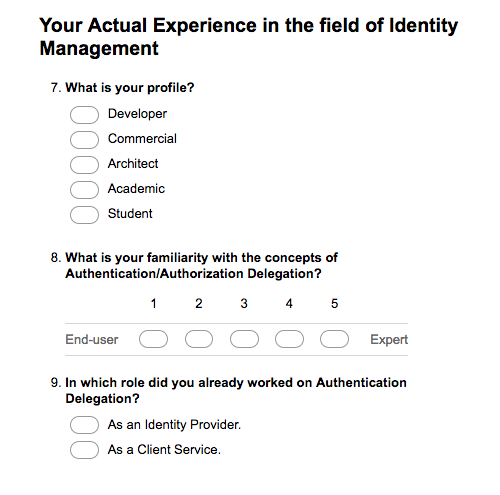
\includegraphics[scale=0.55, angle =90 ]{images/surveyBzhCamp2}
    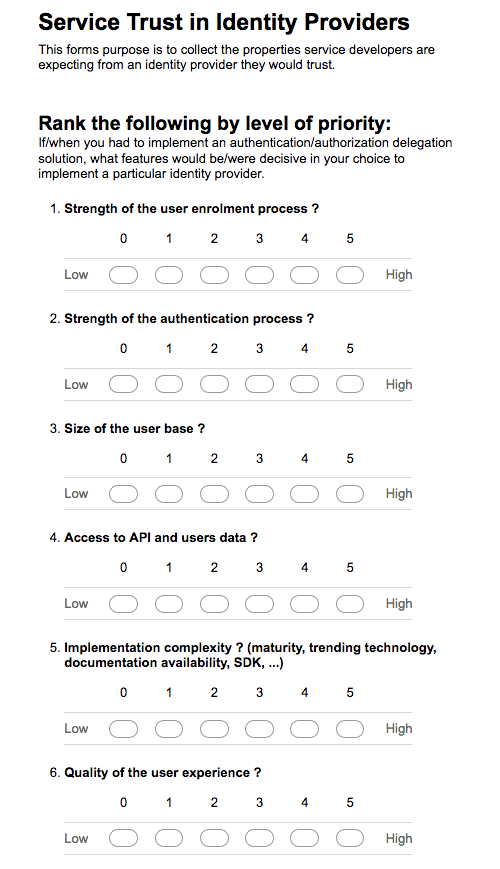
\includegraphics[scale=0.55, angle =90 ]{images/surveyBzhCamp1}
    \caption{BreizhCamp Developer Survey}
    \label{bzhCamp}
\end{figure*}

We conducted a survey during the BreizhCamp 2017, a regional conference targeted at developers from local information technology companies.
During this conference we distributed questionnaire (see Figure~\ref{bzhCamp}) on tables and at our own exposition booth~\footnote{We participated to the BreizhCamp as members of the reThink project which was sponsoring the event.}.
The questionnaire consists in rating the value of six properties of \gls{idp} in the developer's opinion from 0 (low value) to 5 (high priority).
The properties to rate are as follows: 
\begin{itemize}
\item The \textbf{strength of the enrolment} process.
\item The \textbf{strength of the authentication} process.
\item A popular \gls{idp} would have a large \textbf{user base size} and allow many users to connect to the developer's website.
\item The ability for the developer's website to access \gls{idp}'s \textbf{\gls{api} and users' data}.
\item The \textbf{implementation complexity}, \ie maturity, trending technology, documentation availability, SDK availability, ...
\item The \textbf{user experience} when enrolling and authenticating with the \gls{idp}.
\end{itemize} 
Participants are also required to rate their experience in the field of identity management.
This allowed us to discard a single commercial profile and only consider answers from technical profiles.
In total, we thus have 24 exploitable surveys.
All considered respondents are at least familiar with identity management as end-users, and most are capable of quoting some protocols.

\begin{figure}
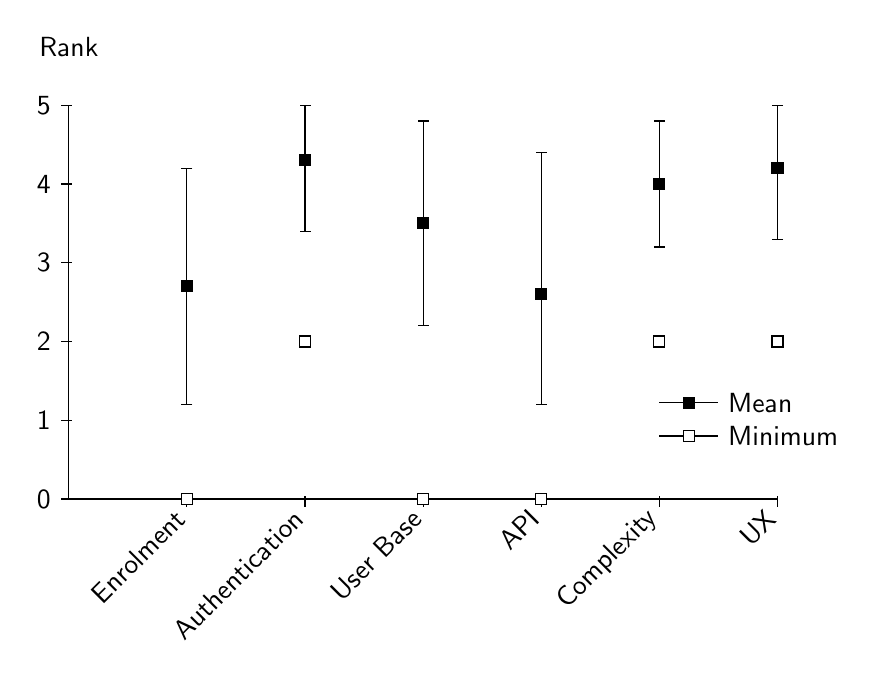
\begin{tikzpicture}[y=1cm, x=1.5cm,font=\sffamily]
     %axis
    \draw (0,0) -- coordinate (x axis mid) (6,0);
        \draw (0,0) -- coordinate (y axis mid) (0,5);
        %ticks
        \draw (1,1pt) -- (1,-3pt)
        node[rotate=45, anchor=east] {Enrolment};
        \draw (2,1pt) -- (2,-3pt)
        node[rotate=45, anchor=east] {Authentication};
        \draw (3,1pt) -- (3,-3pt)
        node[rotate=45, anchor=east] {User Base};
        \draw (4,1pt) -- (4,-3pt)
        node[rotate=45, anchor=east] {API};
        \draw (5,1pt) -- (5,-3pt)
        node[rotate=45, anchor=east] {Complexity};
        \draw (6,1pt) -- (6,-3pt)
        node[rotate=45, anchor=east] {UX};
        
%        \draw (8,1pt) -- (8,-3pt)
%        node[rotate=45, anchor=east] {Experience};
        
         \draw (1pt,0) -- (-3pt,0) 
             node[anchor=east] {0};
         \draw (1pt,1) -- (-3pt,1) 
             node[anchor=east] {1};
         \draw (1pt,2) -- (-3pt,2) 
             node[anchor=east] {2};
         \draw (1pt,3) -- (-3pt,3) 
             node[anchor=east] {3};
         \draw (1pt,4) -- (-3pt,4) 
             node[anchor=east] {4};
         \draw (1pt,5) -- (-3pt,5) 
             node[anchor=east] {5}; 
    %labels      
    %\node[below=0.8cm] at (x axis mid) {MOPS};
    \node[above=3cm] at (y axis mid) {Rank};

    %plots
    \draw plot[only marks, mark=square*]
        coordinates {
        (1,2.7) (2,4.3) (3,3.5) (4,2.6) (5,4.0) (6,4.2) %(8,3.4)%    +- (1.5) 
        };
    \draw plot[mark=-] 
        coordinates {(1,1.2) (1,4.2) };
    \draw plot[mark=-] 
        coordinates {(2,3.4) (2,5)};
    \draw plot[mark=-] 
        coordinates {(3,2.2) (3,4.8) };
    \draw plot[mark=-] 
        coordinates {(4,1.2) (4,4.4)};
    \draw plot[mark=-] 
        coordinates {(5,3.2) (5,4.8)};
    \draw plot[mark=-] 
        coordinates {(6,3.3) (6,5)};
        
%    \draw plot[mark=-] 
%        coordinates {(8,2.5) (8,4.3)};
    
    \draw plot[only marks, mark=square*, mark options={fill=white}]
        coordinates {
        (1,0) (2,2) (3,0) (4,0) (5,2) (6,2)%    +- (1.5) 
        };
    %legend
    \begin{scope}[shift={(5,0.8)}] 
    \draw (0,0) -- 
        plot[mark=square*, mark options={fill=white}] (0.25,0) -- (0.5,0) 
        node[right]{Minimum};
    \draw[yshift=\baselineskip] (0,0) -- 
        plot[mark=square*] (0.25,0) -- (0.5,0)
        node[right]{Mean};
    \end{scope}
\end{tikzpicture}
\caption{Mean, minimum, and standard deviation of the trust survey results.}
\label{fig:trustSurvey}
\end{figure}

Figure~\ref{fig:trustSurvey} shows the minimum, mean, and standard deviation for each parameter of our survey.
We observe a separation of parameters into two main categories:

The first category regroups properties with a high-value and a low standard deviation: \ie authentication strength, implementation complexity, and user experience.
All parameters in this categories demonstrate a minimum rank of 2, a high mean value close to 4, and a standard deviation under 1.
In our opinion, this shows that a consensus from developers exists on the importance of these properties.
This is easily explained as developers have all in common the core task of implementing practical and secure websites, with library they are able to use.

On the contrary, enrolment strength, user base, and access to \gls{api} all show a low value and a high standard deviation.
The enrolment strength and access to \gls{api} parameters have a low mean value of 2.6, and a high standard deviation of 1.5 and 1.8 respectively.
The need for access to an API is highly dependent on the website use-case, which may explain the absence of consensus.
Enrolment strength is also dependent on use case, but from discussions with participants who completed the survey at our booth we also believe that this property may not be as well understood as the authentication strength.
Finally, in the low-value category, we can further distinguish the importance of the user base which shows a higher mean of 3.5 and lower deviation of 1.3.
This may indicate an important but not critical property.
Supposing a developer would like to implement multiple \gls{idp}, even with small user-base, this property would enter in conflict with the quality of the user experience and with the implementation complexity, which are clearly higher priority properties.

Based on our results, we argue that a solution to let users choose their own \gls{idp} should preserve a simple user experience, and ease the implementation complexity.
Whether the website needs to trust the \gls{idp} remains an open question.
On one hand, the enrolment process is not seen as a priority, which may mean that self-asserted identities may not be a problem for some websites.
On the other hand, the authentication strength is clearly a top priority.
We thus also argue that a solution to let users choose the \gls{idp} should probably let websites request trusted \gls{idp} or \gls{aal}.

%\clearpage

\invisiblesection{Summary}
\label{sec:c1Summary}
\vspace*{3cm}

\blockmargin%
\hspace{-\marginparwidth}\hspace{-\marginparsep}
\makebox[\overflowingheadlen][l]{
\begin{minipage}{\overflowingheadlen}

\begin{mdframed}[style=C1Frame,frametitle={\ref{sec:c1Summary}~Summary}]

The WebRTC security architecture~\cite{I-D.ietf-rtcweb-security-arch} claims that trust in the signalling layer can be replaced by trust in the \gls{idp}.
However, in our state of the art (see Chapter~\ref{sota}) we did not observe research considering the \gls{idp} as a potential threat in WebRTC scenario.
In this chapter, our contribution was to study additional privacy implications focusing on the WebRTC identity architecture and on the role of the \gls{idp}.

\medskip

We first presented our implementation of the WebRTC identity architecture and in the particular the integration of the \gls{idp} Proxy component with the \gls{oidc} protocol.
This work reveals that while \gls{oidc} facilitates the creation and signature of WebRTC identity assertion its integration is not straightforward.
In particular, although WebRTC offers an abstract authentication delegation interface it is not particularly suited to manage authorization delegation.
We thus answer to RQ1.1 by showing additional privacy risks that \gls{idp} should take in consideration to implement the WebRTC identity architecture.
We also show how the \gls{idp} can compromise users' privacy without their explicit consent.
The central role and responsibility of \gls{idp} in the web ecosystem is reinforced by their inclusion in WebRTC call setup.

\medskip

We then focused on answering RQ3 to find if we can let users chose actors they trust to participate in the communication setup.
Previous studies reported that users are presented with a limited choice of \gls{idp} when authenticating on the Web.
We conducted a survey of the top-500 website's usage of OAuth~2 and \gls{oidc} to identify possible reasons for this situation.
We classified \gls{rp} by the types of authorization they request to users.
Our results show that a majority of \gls{rp}, 58\% of 103, do not require specialised data.
Although \gls{oidc} proposes standardised profile claims, scopes, endpoint, and data format, we observe that it is implemented by only a few \gls{idp}.
Similarly, \gls{oidc} offers optional dynamic discovery and registration of \gls{rp} but these features are not implemented at all on surveyed \gls{idp}.
That \gls{rp} and \gls{idp} require pre-established trust relations could explain this lack of implementation.
As we focused our survey on interactions observable from the user's browser it does not allow us to answer on that matter.
To further investigate this question, we believe that it should be directly asked to the professional responsible for the deployment of \gls{idp} and \gls{rp} alike.
Finally, we conducted a survey on developer to identify important \gls{idp}'s properties in the developer's opinion.
Our results show a consensus on the need for a strong authentication and well-crafted user experience but not on other properties.
We answer on RQ3.1 and RQ3.2 that while technical solutions for allowing users to choose their \gls{idp} exist, these are not implemented by \gls{idp} and \gls{rp} alike.

\end{mdframed}

\end{minipage}
}
\unblockmargin